\chapter{光的连续谱}
\section{恒星视差}
恒星视差被用于距离测量,这种方法被称为{\bf 三角视差}

\begin{figure}[hbt]
  \centering
  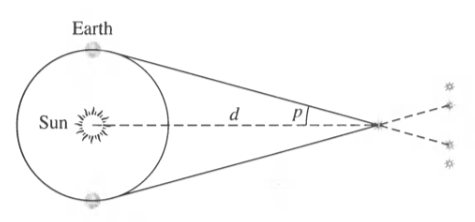
\includegraphics[width=6cm]{chapters/03/parallax}
  \caption{恒星视差,$d=1/p''\mathrm{pc}$}
  \label{fig:parallax}
\end{figure}

如图\ref{fig:parallax}所示,当地球运行到公转轨道的两端时,会观测到目标恒星的位置相对背景星空发生了变化,这种变化体现在天球坐标
(\autoref{sec:celestial})的变化上,即坐标差$p$,通过三角形几何关系,可以得到目标恒星的距离$d$,从而定义秒差距:
\begin{equation}
  d=1/p''\mathrm{pc}
\end{equation}

单位换算:$1\;\mathrm{pc}\approx
3.26\;\mathrm{ly}$,$1\;\mathrm{ly}\approx9.46\times10^{15}\;\mathrm m$

\section{星等}
古希腊的喜帕恰斯(Hipparchus)定义了{\bf 视星等}$m$,且天空最亮的恒星为$m=1$,肉眼看到最暗的恒星为$m=6$。现代观测设备能够定量精确地测量恒星的{\bf 辐射流量}$F$,发现相差5个星等对应辐射流量差100倍,于是得到关系:
\begin{equation}
  m_1-m_2=-2.5\log_{10}\left({F_1\over F_2}\right)
  \label{eq:magnitude}
\end{equation}

地球上测得的太阳的辐射流量称为{\bf 太阳辐照度},或太阳常数:$F={L_\odot \over 4\pi r^2}=1365\;\mathrm{W\;m^{-2}}$

视星等只能观测属性,无法表征恒星本身的发光能力,因此定义当恒星处于10pc处时的视星等为{\bf 绝对星等}$M$,可得到{\bf 距离模数}:
\begin{equation}
  m-M=5\log_{10}\left({d\over 10\;\mathrm{pc}}\right)
  \label{eq:module}
\end{equation}

{\bf \textcolor{red}{注:星等概念注意理解,才能灵活运用}}

\section{黑体辐射}
一个理想的发射源也应该吸收所有入射到其表面上的光,然后再以特征谱的形式辐射出来,这种理想发射源称为{\bf 黑体},相应的辐射称为{\bf 黑体辐射}
\begin{figure}[hbt]
  \centering
  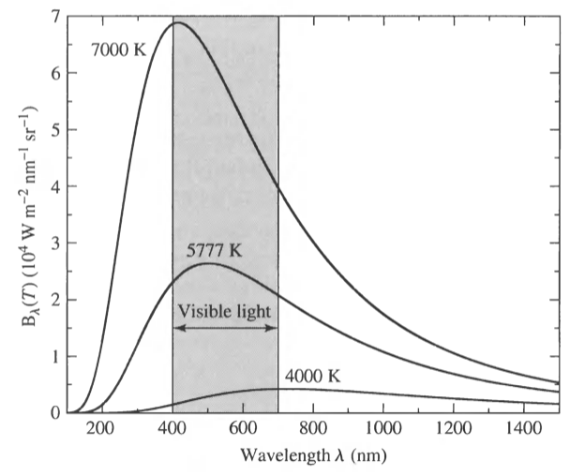
\includegraphics[width=6cm]{chapters/03/blackbody}
  \caption{黑体的光谱}
  \label{fig:blackbody}
\end{figure}

如图\ref{fig:blackbody}所示,黑体谱应该是覆盖全波段的连续谱,但是辐射强度随波长呈一定分布,峰值波长(频率)满足{\bf 维恩位移定律}:
\begin{equation}
  \lambda_\mathrm{max}T\approx0.0029\;\mathrm{m\;K}
\end{equation}

图\ref{fig:blackbody}的黑体谱可以用{\bf 普朗克公式}来描述:
\begin{equation}
  B_\lambda(T)={2hc^2/\lambda^5 \over e^{hc/\lambda kT}-1}
  \label{eq:planck}
\end{equation}

或频率形式:
\begin{equation}
  B_\upsilon (T)={2h\upsilon^3/c^2 \over e^{h\upsilon/kT}-1}
\end{equation}

黑体辐射的光度可用{\bf 斯特藩-玻尔兹曼定律}描述:
\begin{equation}
  L=4\pi R^2\sigma T^4_e
  \label{eq:stefan}
\end{equation}

尽管恒星并不是理想黑体,但是依然可以使用式\ref{eq:stefan}来定义恒星表面的{\bf 有效温度}$T_e$

\section{色指数}
一颗恒星全波段测量得到的星等称为{\bf 热星等(bolometric magnitudes)},记为$m_{bol}$和$M_{bol}$

观测时,往往使用滤光片来使特定波段的光透过,从而精确测量恒星的颜色,滤光片的带宽和中心频率由制作时随需求确定,但有时也用统一标准:
\begin{itemize}
  \item U,紫外星等,中心波长365\;nm,有效带宽68\;nm
  \item B,蓝光星等,中心波长440\;nm,有效带宽98\;nm
  \item V,可见光星等,中心波长550\;nm,有效带宽89\;nm
\end{itemize}

一颗恒星不同波段的星等之差称为{\bf 色指数(color index)},如色指数$B-V$的值越小,说明恒星在$B$波段越亮

热星等和可见光星等的差称为{\bf 热改正(bolometric correction) $BC$}:
\begin{equation}
  BC=m_\mathrm{bol}-V=M_\mathrm{bol}-M_V
  \label{eq:bc}
\end{equation}

现实中无法测量恒星的热星等,但是可以通过式\ref{eq:bc}将光星等+热改正来得到热星等

由式\ref{eq:magnitude}可推得对应波段的星等:
\begin{equation}
  U=-2.5\log_{10}\left(\int_0^\infty F_\mathrm\lambda S_U d\lambda\right)+C_U
\end{equation}

其中$S_U$是响应函数,用于描述入射光的比率,和望远镜的镜面反射率有关,计算时可考虑在有效带宽内为1,有效带宽外为0;$C_U$是一个常数。

上式类比到其他波段可得色指数:
\begin{equation}
  U-B=-2.5\log_{10}\left({B_{365}\Delta\lambda_U \over B_{440}\Delta\lambda_B}\right)+C_{U-B}
\end{equation}

\begin{figure}[hbt]
  \centering
  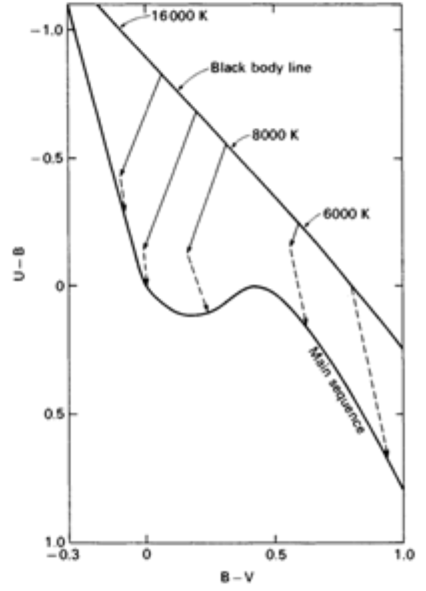
\includegraphics[width=6cm]{chapters/03/CC}
  \caption{双色图,从中可以看出恒星并不是严格的黑体谱,一些特定的发射线会导致特定波段的光强偏离黑体谱,从而出现图中的虚线和实线(氢原子巴尔末线系)箭头所导致的偏差。}
  \label{fig:cc}
\end{figure}
